\subsection{\texorpdfstring{Signal ${E\!\!/}_{\!\mathrm{T}}$  Modeling}{Signal ET Modeling}}
\label{sec:WsignalMETtemplate}

The $\Wln$ signal is extracted with methods that employ
simulation predictions of the $\MET$ distribution in signal events.
These predictions
rely on the modeling of the vector-boson recoil and detector effects that
can be difficult to simulate accurately. Discrepancies could result
from deficiencies in the modeling of the
calorimeter response and resolution, and from an incomplete description of
the underlying event.
% and from simplifications made in the simulation of pile-up.
These residual effects are addressed using corrections
determined from the study of Z-boson recoil in data, discussed in the following paragraph.

The recoil to the vector boson is defined as the negative of the vector
sum of transverse energy vectors of all particles reconstructed with the PF algorithm
in W and Z events, after subtracting the contribution from the daughter lepton(s).
The recoil is determined for each event in $\Zll$ data and simulated $\Zll$
and $\Wln$ samples.
We fit the distributions of the recoil components (parallel and perpendicular to the
boson p$_T$ direction) with a double Gaussian, whose mean and width vary with the boson
transverse momentum.
For each sample, we fit polynomials to the extracted mean and width of the recoil
distributions as functions of the boson transverse momentum.
The ratios of data to simulation fit-parameters from the $\Zo$ samples are used as scale
factors to correct the polynomials parameters of the W simulated recoil curves.
For each $\Wo$ simulated event, the recoil is replaced with a value drawn from the
distribution obtained with the corrected parameters corresponding to the $\Wo$ p$_T$.
The $\MET$ value is calculated by adding back the energy of the $\Wo$ lepton.
%We fit the recoil distributions whose mean and width vary with the boson transverse
%momentum. For each sample, we fit polynomials to the extracted means and widths of the recoil
%distributions as functions of the boson transverse momentum.
%The ratios of data to simulation fit parameters from the $\Zo$ samples are used as
%scale factors to correct the simulated $\Wo$ recoil curves. The recoil in simulated $\Wo$ events
%is replaced with the values drawn from the corrected W recoil distributions,
%adding the energy of the W leptons back to recalculate the $\MET$ value for each event.
The energy of the lepton used in the
calculation is corrected for the energy-scale and resolution effects.  Statistical
uncertainties from the fits are propagated into the $\MET$ distribution as systematic
uncertainties.  An additional systematic uncertainty is included to account for possible
differences in the recoil behavior of the W and Z bosons.

The same strategy is followed for the recoil corrections in the electron and muon analyses.
As an example, Fig.~\ref{fig:Recoil} (left) shows the effect of the recoil
corrections on the $\MET$ shape for simulated events in the electron channel, while Fig.~\ref{fig:Recoil} (right)
shows the uncertainty from the recoil method propagated to the corrected $\MET$ shape
of $\Wen$ events. The distribution of the residuals, $\chi$, is shown at the bottom of each plot,
where $\chi$ is defined as the per-bin difference of the two distributions, divided by the
corresponding statistical uncertainty. The same definition is used throughout this paper.

The systematic uncertainties on the signal $\MET$ shape are propagated as systematic
uncertainties on the extracted signal yield through the fitting procedure.
Signal shapes are determined for the W$^+$ and W$^-$ separately.

%%%%%%%%%%%%%%%%%%%%%%%%%
\begin{figure}
\begin{center}
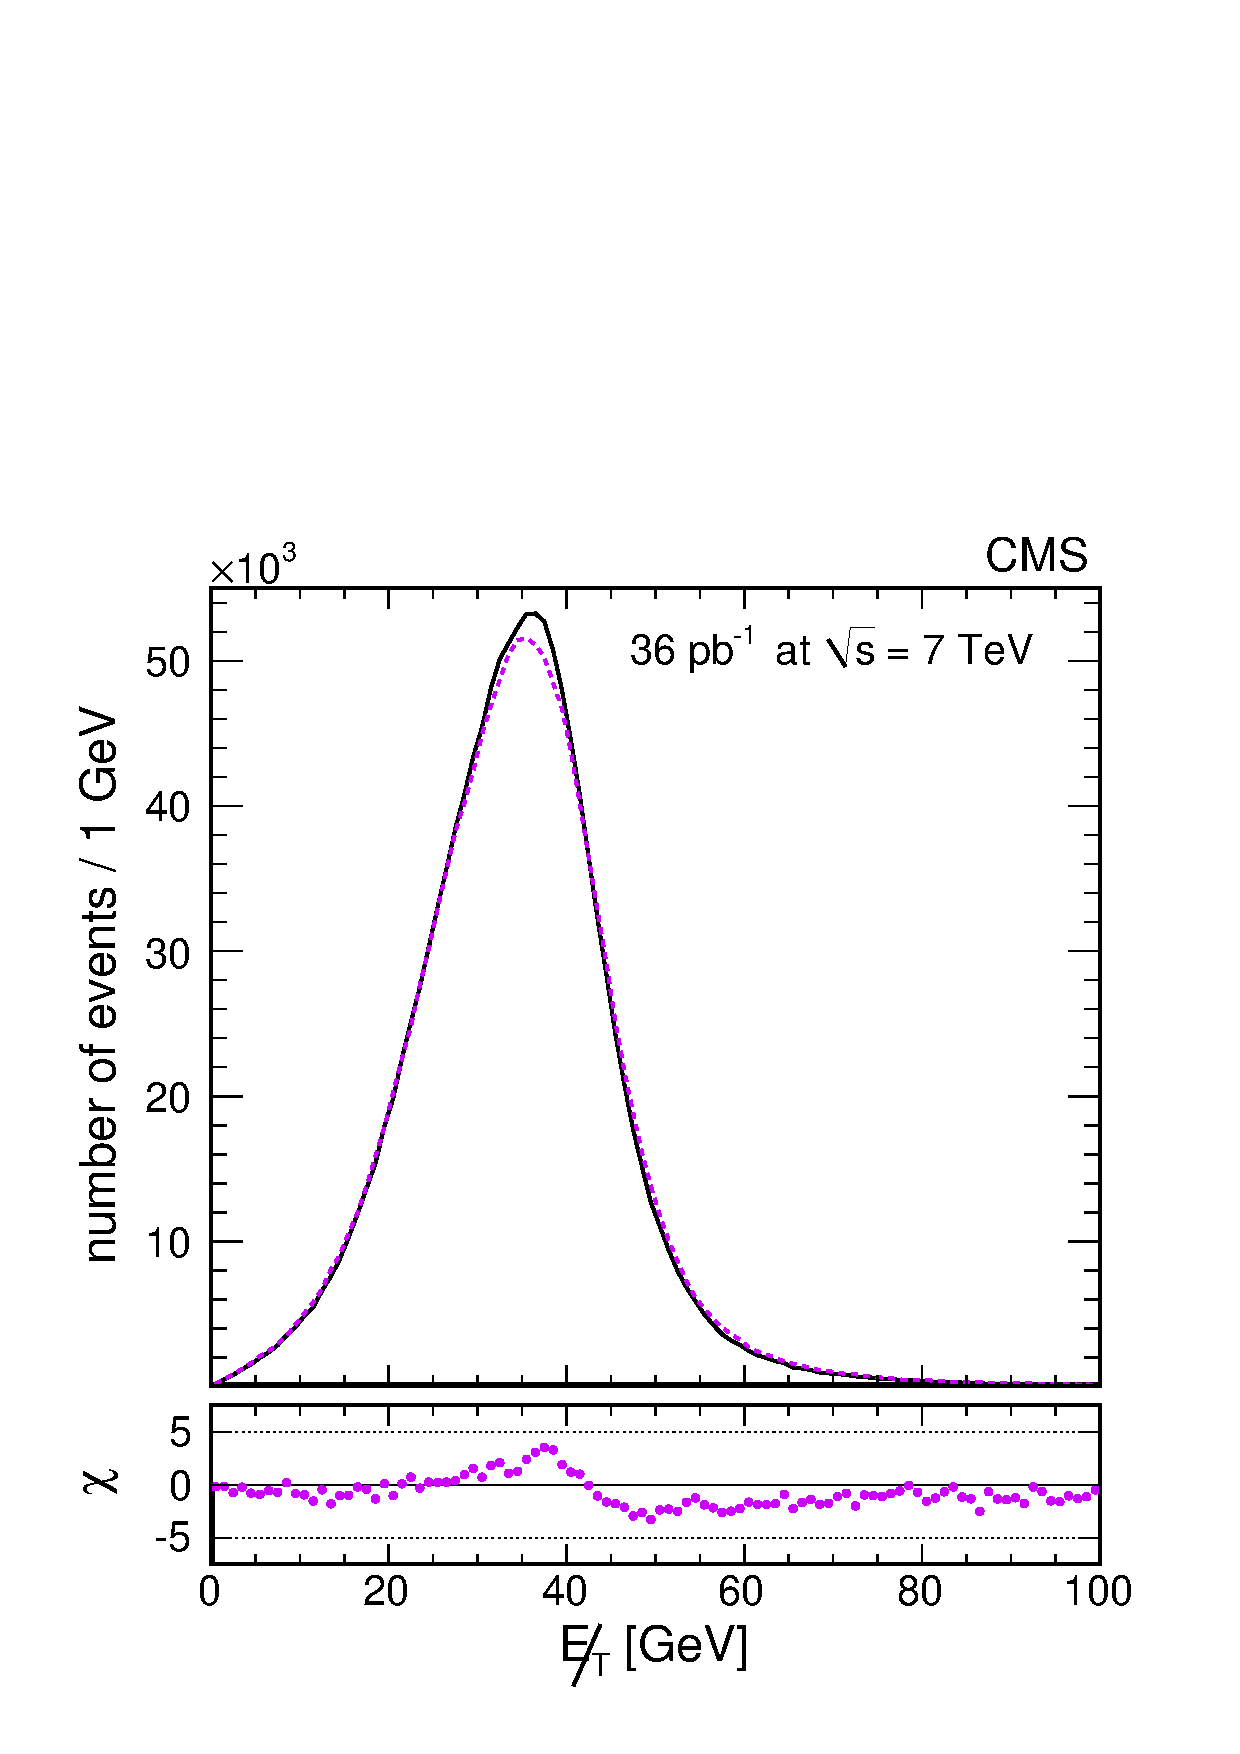
\includegraphics[width=0.48\textwidth]{figs/beforeANDafter.pdf}
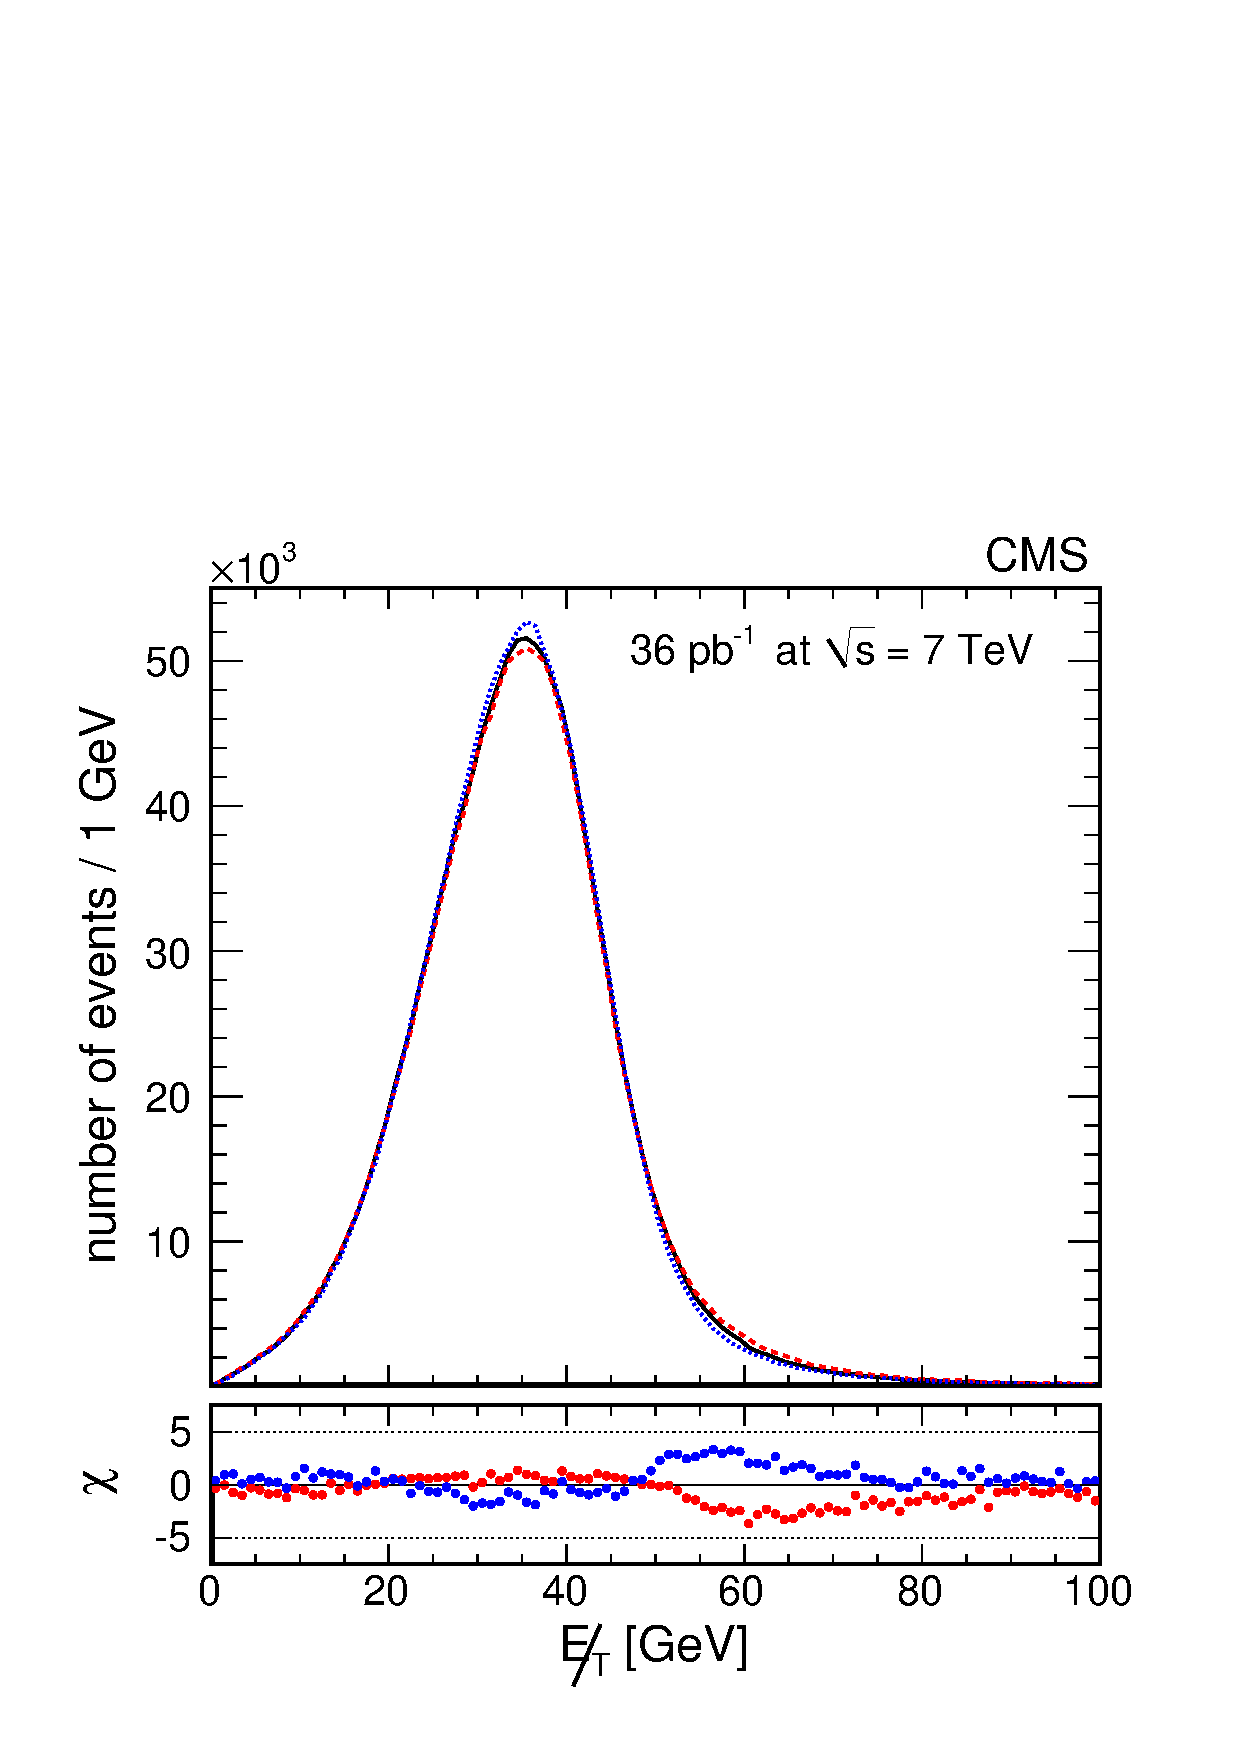
\includegraphics[width=0.48\textwidth]{figs/upANDdown.pdf}
\caption{ \label{fig:Recoil}
Left: simulated $\MET$ distribution in $\Wen$ events before (continuous black line)
and after (dashed red line) recoil corrections.
Right: the uncertainties from the recoil method propagated
to the corrected $\MET$ shape of $\Wen$ events (continuous black line, identical to the dashed
red line on the left-hand side plot) are presented with the red-dashed and blue-dotted lines.
These two shapes are obtained when the recoil systematic uncertainties are varied
by one standard deviation.
At the bottom of each plot is shown the distribution of the residuals, $\chi$, defined
as the per-bin difference of the two distributions, divided by the
corresponding statistical uncertainty.
}
\end{center}
\end{figure}
%%%%%%%%%%%%%%%%%%%%%%%%%
